In this chapter a survey of pervasive healthcare applications is presented. In order to gain a greater understanding of which are the building blocks of an \acf{IoT} system, a reference model is also presented.

\section{Internet of Things}

\subsection{What is IoT?}

\acl{IoT} (or \acs{IoT}) is an emerging communication paradigm, often hailed as the driver of the Fourth Industrial Revolution \cite{Aceto2020}. \bigskip

The definition of this concept has evolved over time with the development of other technologies such as data analytics, embedded systems, etc. Nowadays it describes a strategy supported on the development of networks of smart devices that exchange and process information through Machine-to-Machine (M2M) communications, usually based on the Internet Protocol (IP). This technology enables ubiquitous systems to gather remarkable amounts of information regarding the surrounding environment, which can later be turned into insight through the usage of data analytics tools, like Machine Learning algorithms. \bigskip

More specifically in the healthcare domain, 

\todo[inline]{To-do: Discuss the potential of IoT technologies and bridge to pervasive healthcare applications (such as in Clinics, Hospitals, Smart Home). Cite articles with references to investments in these areas.

- smart systems enable continous patient monitoring
}

\section{A Reference Model for Pervasive Healthcare Applications}

In order to develop an IoT system, it is crucial to design it based on a reference model. A reference model provides a general structure (or a ``template'') for designing systems, thus enabling the comprehension of these complex systems by breaking them down into simple and distinct functional layers, while also defining some common terminology used in its domain.\bigskip

In 2014 the \acs{IoT} World Forum (IoTWF) architectural committee published an \acs{IoT} architectural reference model, composed by seven layers as shown in figure \ref{fig:iotwf-referencemodel}. This model provides a simple and clean functional view into the different components of an \acs{IoT} system without restricting the scope or locality of its components. However, from a hardware perspective, in this work we will restrict our focus to the most common approach taken by investigators, using 3 different components: 

\begin{itemize}
    \item \textbf{Endpoint} or \textbf{edge} nodes (corresponding to Layer 1), which interact with the physical world, capturing data.
    \item \textbf{Gateway} devices (Layers 2-3), which connect to multiple \textbf{edge} nodes, filtering and aggregating the data generated by these, while relaying it to a central server; 
    \item \textbf{Central} server (Layers 4-6), which is responsible for collecting, storing and analyzing the captured data in order to provide users with valuable insight;
\end{itemize}

While this model can be used to develop IoT systems for any industry (from agriculture to smart cities), in the context of the dissertation we will focus on pervasive healthcare applications and its enabling technologies. 

% \todo[inline]{To-do: Make images that summarize key points of each layer (by adapting original images from Cisco documentation?)}

\begin{figure}[H]
    \centering
    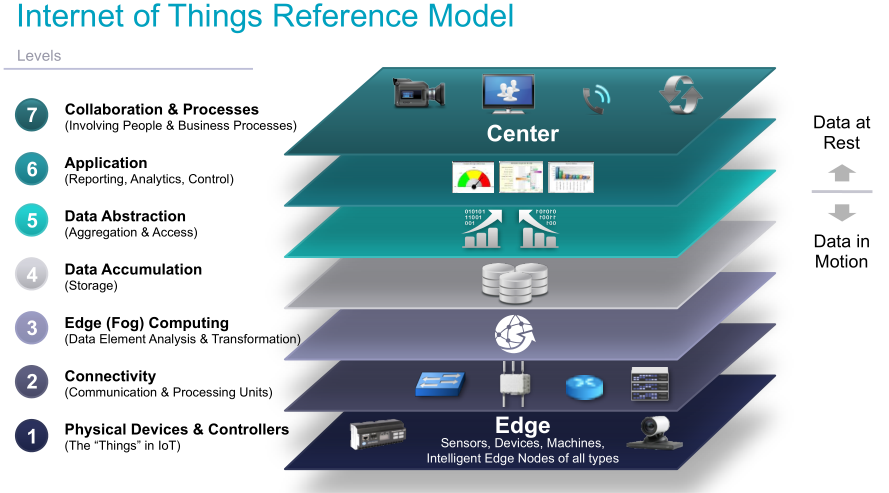
\includegraphics[width=0.85\linewidth]{images/iotwf-referencemodel.png}
    \caption[IoT reference model published by IoTWF.]{IoT reference model published by IoTWF. Source: \cite{Cisco2014}.}
    \label{fig:iotwf-referencemodel}
\end{figure}

\subsection{Layer 1: Physical Devices and Controllers}
\label{sec:iot-model-layer1}

\todo[inline]{To-do: Review this section later.}
The first layer of the model is the physical devices and controller layer. This layer houses the ``things'' in the \acl{IoT}: the endpoint devices composed of sensors and actuators that perceive and interact with the physical world. Through those interactions, the devices generate data, which is then sent across the network for analysis and storage. \bigskip

When designing an \acs {IoT} network, the first step should be to analyze the mobility and data requirements of the system \cite{10.5555/3161403}. \textbf{Mobility} describes the devices' ability to move and, if it is able to, how frequently it does so. \textbf{Data} requirements describe how much data is generated and transmitted by each device per unit of time, and how critical is it to the operation. Simpler health monitoring applications can include a single temperature or heart rate sensor while more complex applications can include pulse oximetry, electrocardiogram (\acs{ECG}), respiration rate sensors, etc. 
\bigskip

With these key requirements established, we can now discuss some other characteristics of the smart devices, like:

\begin{itemize}
    \item \textbf{Power source}: This classification describes if the device has an internal energy supply powering the device or if it has continuous power delivery from an external source. If the device must be mobile, it will require a portable power source, a battery. Battery-powered devices are not bound to a single location, but the finite energy source constrains the device's energy consumption and lifetime, leading to limited memory, computation and connectivity capabilities. 
    \item \textbf{Transmission range}: This classification describes how far away the devices can communicate. In healthcare, these usually have short transmission ranges. For example, a fitness band that communicates with a smartphone will be at most located a few meters from it. 
\end{itemize}

In order to properly design these devices, it is necessary to understand what problems currently reside within clinical environments. Today, hospitalized patients need to be wired to various measurement instruments when continuous biomonitoring is required. This confines the patients to their beds, restricting their mobility, and may also cause skin irritations and infections, aggravating their discomfort and deterioration of their health condition \cite{Darwish2011}. Moreover, the detachment of electrodes from the patient's body, provoked by patient's movements, is one of the main sources of false alarms. These require immediate attention from the hospital staff, contributing to their exhaustion and may ultimately result in the desensitization to the alarms, reducing their response time to real emergencies \cite{DursunErgezen2020}. Wearable, wireless, and non-intrusive devices can to minimize these issues to a large extent, and are seen as one of the key components of \acs{IoT}-based healthcare systems \cite{Baker2017}.  \bigskip

In recent years there has been remarkable progress on the development of wearable devices, driven by recent technological breakthroughs in the miniaturization of sensors and microfabrication processes \cite{Adame2018}. From the literature, we can classify the sensors used in these devices in 3 distinct categories based on information that can be extracted from them, as shown in table \ref{tab:layer1-sensors}:

\begin{itemize}
    \item Monitoring the patient's biosignals, used for evaluating the patient's health condition.
    \item Monitoring the patient's activity or motion, used for detecting fall events, determining the patient's location and travelled distance, estimating the patient's body posture, etc.
    \item Monitoring the patient's environment, mainly used for assessing environmental hazards, \textit{e.g.} gas leaks in a patient's home or an industrial workplace.
\end{itemize}

\begin{table}[H]
    \centering
    \begin{tabular}{l|l}
        \textbf{Type of monitoring} & \textbf{Type of sensors used} \\ 
        \hline
        \multirow{3}{*}{Vital Signs Monitoring} & Body Temperature, Heart Rate, Heart Rate Variability, \\ & Respiratory Rate, Galvanic Skin Response, Blood Pressure, \\ & Pulse Oximetry, \acs{ECG}, Glucose Level Sensors \\ \hline
        \multirow{2}{*}{Activity Monitoring} & Accelerometer, Gyroscope, Magnetometer, Ultrasound Sensors,\\ & \acf{RFID} Tags\\
        \hline
        \multirow{1}{*}{Environmental Monitoring} & Air Temperature, Humidity, Hazardous Gas Sensors \\
    \end{tabular}
    \caption[List of sensors commonly used in pervasive healthcare applications]{List of sensors commonly used in pervasive healthcare applications, adapted from \cite{MinhDang2019}.}
    \label{tab:layer1-sensors}
\end{table}

\subsection{Layer 2: Connectivity}
\label{sec:iot-model-layer2}

\todo[inline]{To-do: Review this section later!!}

The second layer of the model focuses on connectivity, on linking the different components of our system, ensuring reliable and timely data transmissions. This includes all communications within the system, which can be split into two categories: communications within the local network (\textit{e.g.} between edge nodes and the gateway devices), and communications between the edge of the local network (\textit{e.g.} gateway devices) and the central server. \bigskip

\subsubsection{Communication Protocols}

Technologies are designed with certain use cases in mind. They drive their development and thus it is natural that each one has their own advantages and disadvantages, depending on their use. For instance, short range wireless protocols are limited by the transmission range, but long range protocols usually have a higher energy consumption, which may be unviable for networks with very constrained devices. Each protocol also defines their own frame format and communicate within certain frequency bands, which may require special licenses. Due to the frequency bands used by UHF \acs{RFID}, metal and water surfaces near the devices introduce great interference in its transmissions due to signal reflections, thus reducing the effective transmission range \cite{Cairo2018}. The figure \ref{fig:communication-protocols} shows some commonly used protocols in \acs{IoT} systems grouped by range. 

\begin{figure}[H]
    \centering
    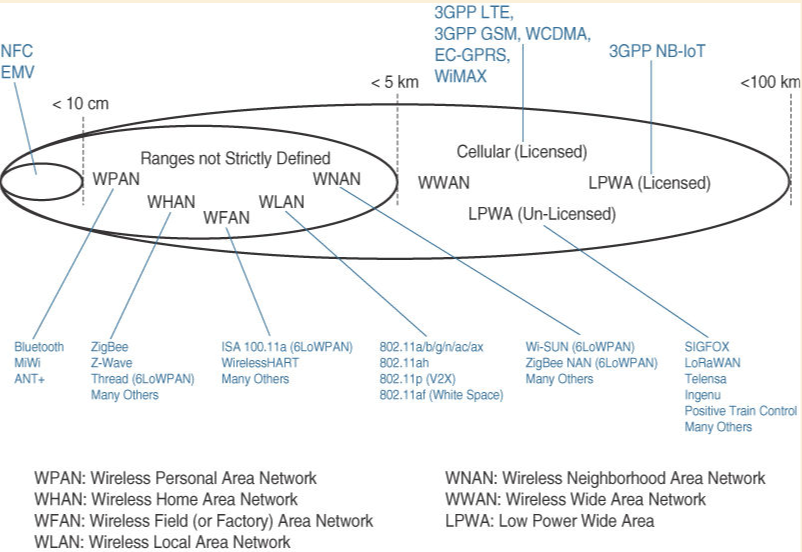
\includegraphics[width=0.85\linewidth]{images/communication-protocols.png}
    \caption[Classification and grouping of various network protocols by range.]{ Classification and grouping of various network protocols by range. Source: \cite{10.5555/3161403}}
    \label{fig:communication-protocols}
\end{figure}

\todo[inline]{To-do: Make new image based on this one.}

Regarding 

\todo[inline]{To-do: Add small comparison of most common protocols WSN used in healthcare? BLE, ZigBee?}

Regarding 

\todo[inline]{To-do: Complete section with short comparison between NB-IoT, LTE? Mention WiFi as the best solution tho }

\todo[inline]{To-do: Complete section with short comparison between MQTT and CoAP}


The choice of the communication protocol is driven by the characteristics of the smart devices, as defined in the first layer. However, we can highlight other key points that affect this decision:

\begin{itemize}
    %\item \textbf{Cost}: The cost of implementing certain protocols may not be economically viable. \acs{RFID} systems are a great example of this. The development of \acs{RFID} tags is inexpensive, but this is offset by the immense cost of the \acs{RFID} readers, which can quickly become unsustainable.
    \item \textbf{Latency}: Certain applications deal with time critical events, for example the detection of health emergencies. In these cases, any delays in the communications can cause great detriment to the patient's well-being, making it crucial to minimize them.
    \item \textbf{Throughput}: The communication protocol should ensure there is enough bandwidth to handle all communications within the designated transmission range. Even within similar technologies, this can vary wildly with the range as seen in figure \ref{fig:communication-protocols-throughput}. 
    \item \textbf{Security}: Security is one of the most important requirements of any system, but this is especially true for healthcare systems. Due to the sensitive nature of the information, it is crucial to secure the information from malicious actors. Communication protocols must implement security mechanisms, such as encryption or data integrity verifications, that ensure the transmissions are not compromised in transit, thus denying third parties the ability to snoop or tamper the transmissions. This issue is studied in depth by \cite{Gope2016}.
    \item \textbf{Interoperability}: To ensure the interoperability of the system it is imperative to choose protocols that are widely accepted and supported by the industry. This also contributes to the longevity of the system, as these will most likely remain supported for longer time periods. %, ensuring maintainability.  
    \item \textbf{Scalability}: This determines how many devices are supported and how many more can be added to the system, thus giving us a measure of the system's flexibility for expanding beyond the initial development. 
\end{itemize}

\begin{figure}[H]
    \centering
    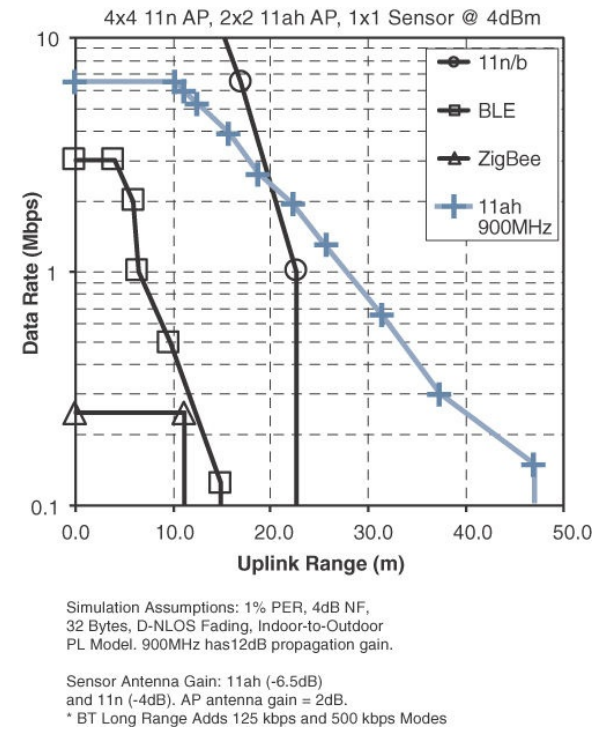
\includegraphics[width=0.55\linewidth]{images/communication-protocols-throughput.png}
    \caption{Throughput versus Transmission range for four WHAN to WLAN communications protocols. Source: \cite{10.5555/3161403}}
    \label{fig:communication-protocols-throughput}
\end{figure}

\subsection{Layer 3: Edge (Fog) Computing}
\label{sec:iot-model-layer3}

\acs{IoT} systems can often have hundreds or even thousands of sensors generating data multiple times per second, 24 hours per day, which can demand an unsustainable amount of network and computing resources. Moreover, certain applications may be time critical, where delays in communication can be very detrimental. To minimize these effects, it is crucial to initiate data processing as close to the edge of the network as possible. This paradigm is usually referred to as ``edge computing'' (when the data processing occurs at the endpoint devices) or ``fog computing'' (when it happens at the edge of local network, \textit{e.g} in ``gateway'' devices). The third layer of the model defines how the system prepares the data for storage and higher level processing for the next layers. The data processing at this stage is generally very limited, mostly focused on ``preprocessing'' the data and handling time critical events. More demanding and thorough analysis should be left to the central server, which holds much greater computing power. The different processes applied at this stage usually are:

\begin{itemize}
    \item \textbf{Filtering}: Assessing if the data should be processed at a higher level. 
    \item \textbf{Formatting}: Reformatting data to ensure consistent formats for higher-level processing.
    \item \textbf{Cleaning}: Reducing data to minimize the impact of data on the network and higher level processing systems.
    \item \textbf{Analysis}: Determining whether data represents a threshold or alert. This is especially relevant for applications that deal with time critical events as seen in the previous section.
\end{itemize}

\subsection{Layer 4: Data Accumulation}
\label{sec:iot-model-layer4}

\todo[inline]{To-do: Review this section later.}

The data that is generated by the edge devices is propagated through the system, moving through each layer with each sensor reading. Up to this point, the model is event driven. However, most applications cannot make use of the data at the rate it is generated. In this layer, Data Accumulation, we define how the system captures the data and stores it, so it becomes usable for applications when needed, providing a transition from event to query-based processing. This includes any issues related with data storage: how the data should be stored (\textit{e.g.} using a relational database, non-relational database, distributed file systems, data compression, etc.), what data should be stored and which should be kept for short-term use, etc.

In healthcare, big data analytics is seen as one of the most promising features of \acs{IoT} applications. However, the massive data collection that is associated with ubiquitous systems causes many issues concerning the processing and storage of data. Cloud platforms are often seen as a solution to this problem \cite{Baker2017}. This is made possible due to the elasticity in allocating, swiftly and inexpensively, computing and storage resources on-demand, adjusting itself to the needs of each application. We can find 3 distinct types of cloud services:

\begin{itemize}
    \item \textbf{Infrastructure as Service (IaaS)}: Provides control over the remote machine (composed of virtual or dedicated hardware), operative system and middleware. This approach gives system designers the highest level of flexibility over the infrastructure, but requires more maintenance.
    \item \textbf{Platform as a Service (PaaS)}: Provides a simple framework for developing applications, where the service provider manages the underlying infrastructure issues such as software updates and hardware maintenance. 
    \item \textbf{Software as a Service (SaaS)}: Provides the finished applications to be used by the end users, in this case health workers, that enable them to work. A simple example is a web-based email service, such as Gmail or Microsoft Outlook. 
\end{itemize}

\begin{figure}[H]
    \centering
    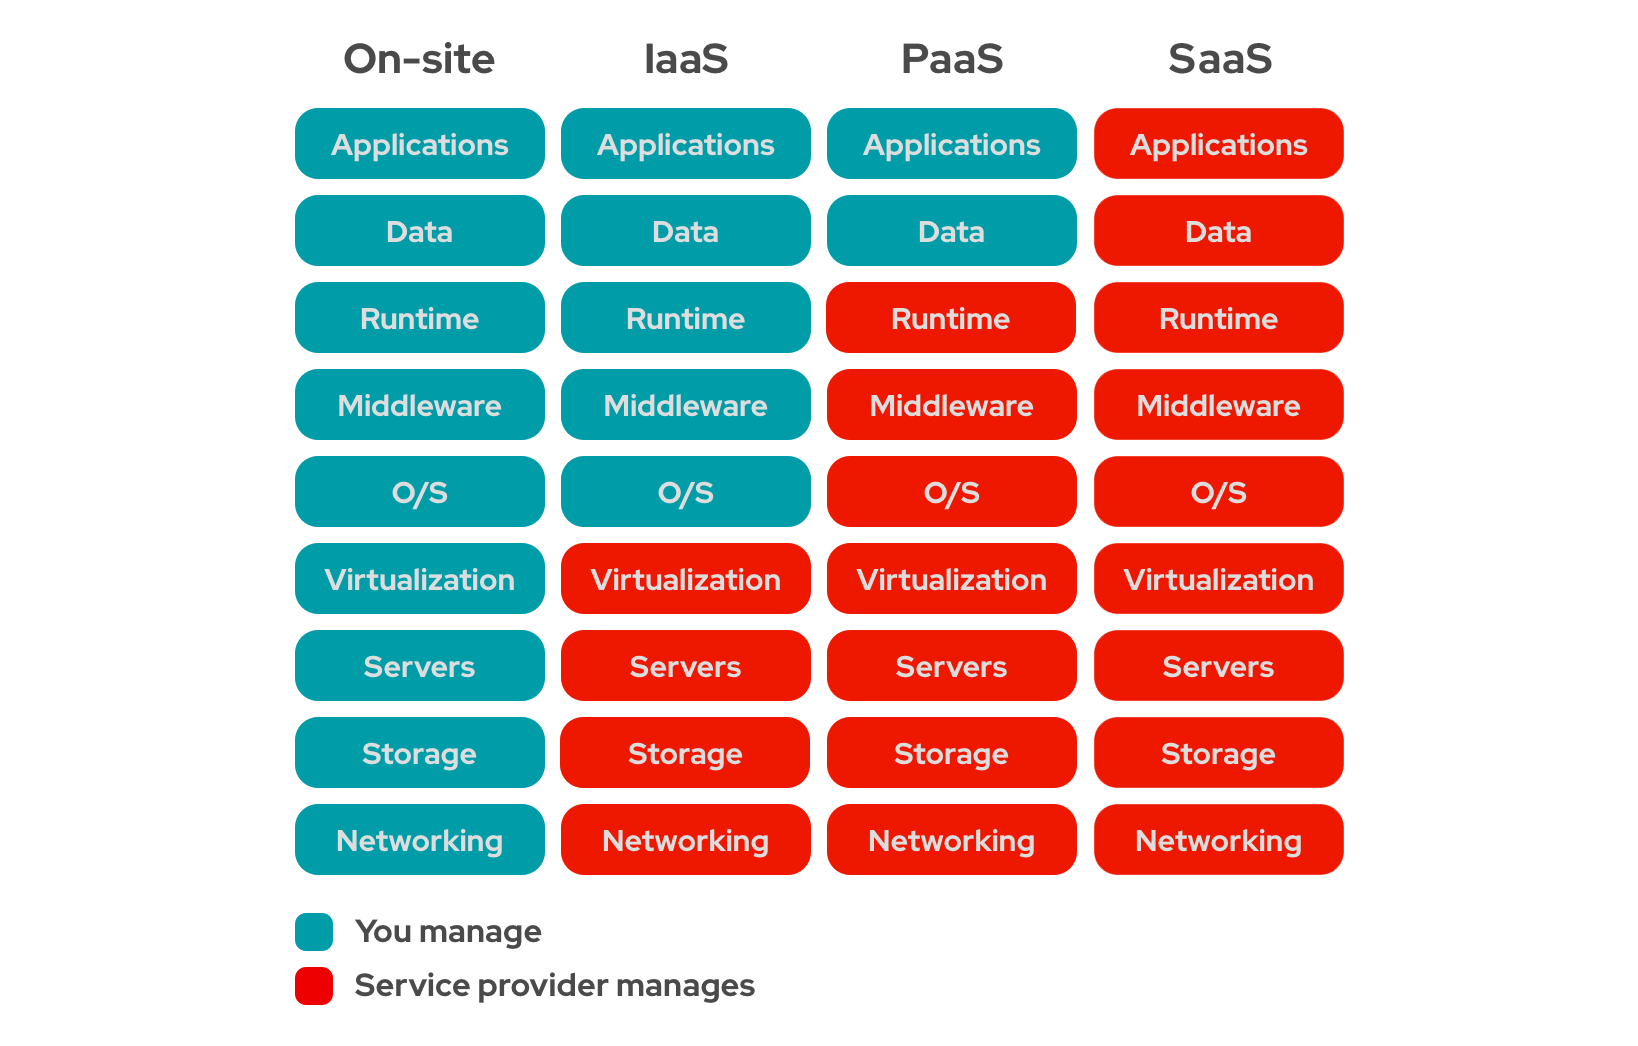
\includegraphics[width=\linewidth]{images/cloud-services.png}
    \caption[Differences between the cloud offerings and on-premise solutions.]{ Differences between the cloud offerings and on-premise solutions. Source: \cite{RedHat2021}}
    \label{fig:differences-between-cloud-services}
\end{figure}

Nonetheless, security and privacy remain as key issues in cloud systems. The information must remain accessible to authorized parties such as healthcare providers, but the patient's health data has to kept private. To solve this, there are two commonly adopted features in the literature:  access control policies and data encryption. Access control policies define who can access the data, by authenticating them (validating the identity of the user) and by authorizing them (ensuring that the user has permissions to perform a given operation). Data encryption ensures that, even if the data is leaked, it is still unreadable to third parties, and therefore the sensitive information remains secure and private.

\subsection{Layer 5: Data Abstraction}
\label{sec:iot-model-layer5}

\todo[inline]{To-do: Review this section later.}

In the previous layer, Data Accumulation, we've defined how the system captures the information. In large scale systems, the collection of data may require the development of multiple concurrent storage solutions, each using different technologies, resulting in a very complex environment. The purpose of this layer is simplify how the applications access the data, to reconcile the different data stores and ensure the information is complete and consistent. 

This is generally accomplished with the development of \acl{API}s (\acs{API}). An \acs{API} is a computing interface that defines a set of rules that ``explain how computers and applications communicate with one another''. \cite{IBMAPI}, acting as an intermediary between different systems and software components. It defines what operations can be performed, how to request them, which are the accepted data types, etc. 

Regarding healthcare services, as patients continuously move around the healthcare ecosystem, their health information must be available, discoverable and understandable to different entities (hospitals, laboratories, pharmacies, etc.). This prompts the digitization of medical files and the development of standards for exchanging these records instantly and securely to authorized users \cite{HL72019}, which are called \acl{EHR}s (\acs{EHR}s). \acs{EHR}s is the digital equivalent of a patient's paper-chart, it contains the patients' full medical history: previous diagnoses, treatment plans, test results, known allergies, among other details. It is now an essential component of health IT. One of the most prominent \acf{FHIR} is a standard data format for exchanging \acs{EHR}s, developed by Health Level Seven International (HL7). HL7 is a non-profit organization involved in the development of international healthcare informatics for over 20 years. \acs{FHIR} builds upon previous data format standards like HL7 v2 and HL7 v3, and is becoming more and more widely adopted within the healthcare industry. 


\subsection{Layer 6: Application}
\label{sec:iot-model-layer6}

\todo[inline]{To-do: Complete section.}

% Interprets data using software application. Applications may monitor, control and provide reports based on the analysis of the data.

The sixth layer is the application layer, where the system proceeds to analyze the data captured and 

% Finally, machine learning to perform diagnostics or provide treatment plans would be extremely valuable in a healthcare context, so a cloud storage framework for healthcare would need to enable value. As all of the characteristics of big data are important to healthcare applications, recent research in this area has focused on storing a wide variety of data generated by voluminous IoT systems in an organized manner that may be useful for later data analysis.

% Centralized and hassle-free collection of data from humans, is a very desired topic in digital health, since it would allow discovery of new digital biomarkers. That is, by acquisition and analysis of electrical/auditory/other physical events of the body, one can find new relationships between certain conditions of the patients and these events [76]. As an example, it is known that dementia has effects on regulation of the body temperature. Therefore, would it be possible to use continuous monitoring of the body temperature and AI to discover Alzheimer development? Although this is not the objective of this project, the proposal makes an important step towards providing large and diverse data to data scientists for analysis. Within this project, we will demonstrate a preliminary example of this ambitious objective, by analyzing 24 hours of data from 3 volunteer who are using a specific drug (i.e. paracetamol or similar), and demonstrate the effect of the drug intake on various parameters, including temperature, emotions, heart rate, blood oxygen, and respiration.

% Level 6 is the application level, where information interpretation occurs. Software at this level interacts with Level 5 and data at rest, so it does not have to operate at network speeds.
% The IoT Reference Model does not strictly define an application. Applications vary based on vertical markets, the nature of device data, and business needs. For example, some applications will focus on monitoring device data. Some will focus on controlling devices. Some will combine device and non-device data. Monitoring and control applications represent many different application models, programming patterns, and software stacks, leading to discussions of operating systems, mobility, application servers, hypervisors, multi-threading, multi-tenancy, etc. These topics are beyond the scope of the IoT Reference Model discussion. Suffice it to say that application complexity will vary widely.
% Examples include:
% ● Mission-critical business applications, such as generalized ERP or specialized industry solutions
% ● Mobile applications that handle simple interactions
% ● Business intelligence reports, where the application is the BI server
% ● Analytic applications that interpret data for business decisions
% ● System management/control center applications that control the IoT system itself and don’t act on the data produced by it.
% If Levels 1-5 are architected properly, the amount of work required by Level 6 will be reduced. If Level 6 is designed properly, users will be able to do their jobs better. Figure 8 depicts Level 6.

\subsection{Layer 7: Collaboration and Processes}
\label{sec:iot-model-layer7}

\todo[inline]{To-do: The Cisco model defines a seventh layer: Collaboration and Processes, but how can one model for it (if it is even possible)?  Should this section be removed entirely, or what should be added to make it more complete? }

The information that is created by the \acs{IoT} yields little value unless it prompts action, which requires people and processes (seventh layer) — this is what differs \acs{IoT} from traditional \acl{IT} systems. The objective is not the application — it is to empower people to work better and more efficiently. The sixth layer (Applications) provides business people the right insight, at the right time, so they can make the right decision. To do this people must be able to communicate and collaborate, which often requires multiple steps and transcends multiple applications \cite{Cisco2014}.

\section{Similar approaches}

% \todo[inline]{To-do: Complete section!  Add introductory paragraph!  Perform a critical analysis of all related work. You should make clear and focus on what is your contributions, and state clearly what is *not* your contributions (i.e. out of the scope of this work). Falta um parágrafo introdutório. O que se vai fazer nesta sub.secção? pq }

% This chapter presents a survey of patrolling, surveillance, navigation and exploration strategies already implemented in the literature. In the last decades, related algorithms for multiple robot teams have piqued the interest of the robotics community, becoming a remarkable growing area. One of the main reasons contributing to this fact is the variety of approaches that these algorithms can comprise. Many authors contributed with studies that involve many different strategies to solve these problems. In this section, some of the background work related to different strategies is presented. The reader will note that it is not imperative to follow just one of these strategies. In fact, most of them result from mixed strategies, though more evident characteristics related to the strategy being discussed are focused in each section.
% <---- Real-time tracking systems ---->

We have thoroughly discussed how \acs{IoT} systems are designed, but so far we have not discussed details of any specific implementation so far. This section presents an overview of \acs{IoT} connected healthcare applications described in the literature, highlighting each of their strengths and weaknesses. \bigskip
%==========================================================================================================================================
%[1] P. Fuhrer and D. Guinard, “Building a smart hospital using RFID technologies,” Eur. Conf. eHealth 2006, Proc. ECEH 2006, pp. 131–142, 2006.
%
%--------------------------
% Physiological & Environmental Signals: (L1) 
% - RFID tag
% Networking Protocols: (L2)
% - RFID (EPC Gen1?), WiFi
% Gateway: (L3)
% - Beaglebone Black
% Data Storage: (L4)
% - MySQL
% e-Health Standards: (L5)
% - None
% Application Features: (L6)
% - Real-Time Tracking System (Patients and Assets)
% Security:
% - Unknown Storage Encryption 
% User Interface:
% - Custom Web application
% Other Notes: 
%------------------------------

In \cite{Fuhrer2006}, one of the first \acs{IoT} applications for healthcare is described. The authors propose a real-time locating system (RTLS) using \acs{RFID} tags called RFIDLocator. These tags are placed in hospital equipment, staff, patients and medical files and by using \acs{RFID} readers placed in strategic locations around the hospital (\textit{e.g.} entrance of rooms, handheld readers), it is possible to track the location of each object. When a \acs{RFID} reader detects a \acs{RFID} tag it communicates this information, using Wi-Fi, to a central server which stores it in a MySQL database. Healthcare workers can then view this information through a web application, which contains a location history of the tagged object. The authors show how RTLS systems can mitigate the risks of patient misidentification, loss or theft of assets and even drug counterfeiting. However, in this article, security and privacy issues are not discussed. Although not stated explicitly, communications between the RFID tags and the RFID readers are assumed to be unencrypted, which means ``unethical individuals could snoop on people and surreptitiously collect data (...) without their knowledge'', even after leaving the hospital if the tags are not removed. This raises serious privacy concerns, as the tags could contain private information that can be detrimental to the patients if revealed. \bigskip

%==========================================================================================================================================
%[2] T. Adame, A. Bel, A. Carreras, J. Melià-Seguí, M. Oliver, and R. Pous, “CUIDATS: An RFID–WSN hybrid %monitoring system for smart health care environments,” Futur. Gener. Comput. Syst., vol. 78, pp. %602–615, Jan. 2018, doi: 10.1016/j.future.2016.12.023.
% 
%--------------------------
% Physiological & Environmental Signals: (L1) 
% - Temperature, Heart Rate, Accelerometer
% Networking Protocols: (L2)
% - RFID (European UHF EPC Gen2), WiFi
% Gateway: (L3)
% - Beaglebone Black
% Data Storage: (L4)
% - MySQL
% e-Health Standards: (L5)
% - None
% Application Features: (L6)
% - Real-Time Tracking System (Patients and Assets), Fall Detection, Vital signs monitoring 
% Security:
% - AES-128 (iot node <-> gateway), WPA-Personal (gateway <-> server)
% User Interface:
% - Custom Web application
% Other Notes: 
% - Ran a hospital trial
%------------------------------

In \cite{Adame2018}, the authors propose a RTLS system that also monitors the patient's vital signs, using a small wristband which holds a low power device equipped with temperature, photoplethysmography (\acs{PPG}), used to obtain the heart rate, and accelerometer sensors, used for detecting fall events. The system can also detect with 70\% accuracy if the patient has fallen, sending an immediate message to the gateway, which will later alert the clinical staff to the emergency. The authors ran a pilot test within hospital premises which was well-received by the clinical staff who praised the system for its intuitiveness and non-intrusiveness, stating that it could be easily integrated into their current \acs{HIS}. However, the authors pointed out some issues related to the usage of \acs{RFID} tags with sensors for patient monitoring. The \acs{RFID} reader powers the \acs{RFID} tags, and when using tags with sensors, the readers need to provide considerably more energy to the tags. The readers must be adjusted to provide enough power, but local regulations limit the transmission power. Regarding e-health standards, the authors did not discuss any protocols for exchanging data such as \acs{FHIR}, which can undermine the integration of the system with existing \acs{HIS}s. \bigskip

%==========================================================================================================================================
%[3] L. Catarinucci et al., “An IoT-Aware Architecture for Smart Healthcare Systems,” IEEE %Internet Things J., vol. 2, no. 6, pp. 515–526, Dec. 2015, doi: 10.1109/JIOT.2015.2417684.
%
%--------------------------
% Physiological & Environmental Signals: (L1) 
% - Temperature, ECG, Accelerometer, Barometric Pressure, Ambient Light
% Networking Protocols: (L2)
% - RFID (European UHF EPC Gen2), 6LowPAN
% Gateway: (L3)
% - TI MSP430F2618, Smartphone
% Data Storage: (L4)
% - 
% e-Health Standards: (L5)
% - None
% Application Features: (L6)
% - Real-Time Tracking System (Patients and Assets), Fall Detection, Vital signs monitoring 
% Security:
% - 
% User Interface:
% - 
% Other Notes: 
% - 
%------------------------------
% \cite{Catarinucci2015}

%==========================================================================================================================================
%[4] T. Wu, F. Wu, C. Qiu, J. M. Redoute, and M. R. Yuce, “A Rigid-Flex Wearable Health Monitoring Sensor Patch for IoT-Connected Healthcare Applications,” IEEE Internet Things J., vol. 7, no. 8, pp. 6932–6945, 2020, doi: 10.1109/JIOT.2020.2977164.
%
%
%--------------------------
% Measured Signals: (L1) 
% - 
% Networking Protocols: (L2)
% - BLE (v4)
% Gateway: (L3)
% - Raspberry Pi 3, Smartphone
% Data Storage: (L4)
% - MySQL
% Data Formats: (L5)
% - 
% Application Features: (L6)
% - 
% Security:
% - AES-128
% Integration with HIS:
% - No
% Other Notes: 
% - 
%------------------------------
%Future Work:
%"Since security is not the focus of this article, the two common security measures are implemented to meet the basic requirements of the following: (...) Security Between Wearable Patches and Gateways (...) Security Measures in Gateways and Cloud Server"
%"In our future work, more edge computing functions on the gateway will be developed for an IoT-connected healthcare platform."

%\todo[inline]{To-do: Review the critical analysis of this article.}

Wu et al. \cite{Wu2020} have developed a system which uses wearable sensor patches to monitor the patients' status. The wearable sensors transmit the different physiological signals (\acs{ECG}, \acs{PPG} and body temperature) to gateways using \acs{BLE}, which can either by fixed (using a Raspberry Pi module) or mobile (using a smartphone app). The gateway exchanges data with the cloud through bridged \acs{MQTT} brokers, after which it is stored in a MySQL database. The data is stored both in the cloud server and in the fixed gateway. The local users can interact with the system through a web-based user interface (UI) using the smartphone or other web browsers in the local area network. However, the usage of local data storage can cause data integrity issues as the system must ensure databases in both the server and gateways are synchronized at all times. This can undermine the scalability of the system, as the redundant data synchronization can become a performance bottleneck in the long term. \bigskip

%==========================================================================================================================================
%[5] C. Doukas and I. Maglogiannis, “Bringing IoT and Cloud Computing towards Pervasive Healthcare,” in 2012 Sixth International Conference on Innovative Mobile and Internet Services in Ubiquitous Computing, Jul. 2012, pp. 922–926, doi: 10.1109/IMIS.2012.26.
%
%
%--------------------------
% Measured Signals: (L1) 
% - 
% Networking Protocols: (L2)
% - BLE (v4)
% Gateway: (L3)
% - Smartphone
% Data Storage: (L4)
% - MySQL
% Data Formats: (L5)
% - Unknown
% Application Features: (L6)
% - 
% Security:
% - AES-128
% Integration with HIS:
% - No
% Other Notes: 
% - 
%------------------------------

In \cite{Doukas2012}, the authors proposed a \acs{IoT} infrastructure that acquires real-time patient data from wearable sensors, using a cloud platform to handle all data processing and storage requirements. The authors have developed a wearable device which takes the form of a sock, designated ``CloudSensorSock''. The CloudSensorSock acquires mobile data, through accelerometer and gyroscope sensors, vital data, through temperature and heartbeat sensors, and contextual information about the patient's environment using air quality ($CO_2$) sensors. It communicates with a mobile app through \acs{BLE}, which acts as a gateway to the cloud server. The authors propose moving the data processing entirely to the cloud server as cloud platforms can scale to the needs of the application with little management and cost. However, this approach may not be viable for time critical applications. As discussed earlier, the latency in the communications between devices and remote servers may have a negative impact on the application, especially since the authors propose using this system for detecting fall events. \bigskip

%==========================================================================================================================================
%[6] eCovig
%
%
%--------------------------
% Measured Signals: (L1) 
% - 
% Networking Protocols: (L2)
% - BLE (v4)
% Gateway: (L3)
% - Smartphone
% Data Storage: (L4)
% - Unknown
% Data Formats: (L5)
% - 
% Application Features: (L6)
% - 
% Security:
% - Unknown
% Integration with HIS:
% - No
% Other Notes: 
% - 
%------------------------------

Recently, and motivated by the COVID-19 pandemic, Raposo et al. \cite{Raposo2021} developed a system called ``e-CoVig'' a low-cost solution for monitoring COVID-19 patients during the quarantine, as shown in Figure \ref{fig:ecovig-architecture}. The data acquisition is performed using a mobile app. To collect physiological data, the authors developed a specialized wearable device that communicates with the mobile app through \acs{BLE}, recording pulse oximetry ($SpO_2$), heart rate, and temperature data. Alternatively, patients can use their own measuring devices, \textit{e.g.} a thermometer, and manually insert the measurements or use Optical Character Recognition (OCR) to automate the in-app insertion of the values. The app can also be used to record audio snippets in order to detect cough and monitor respiratory activity. Unfortunately, the lack of e-health standards hinders its integration with external healthcare systems. 

\begin{figure}[H]
    \centering
    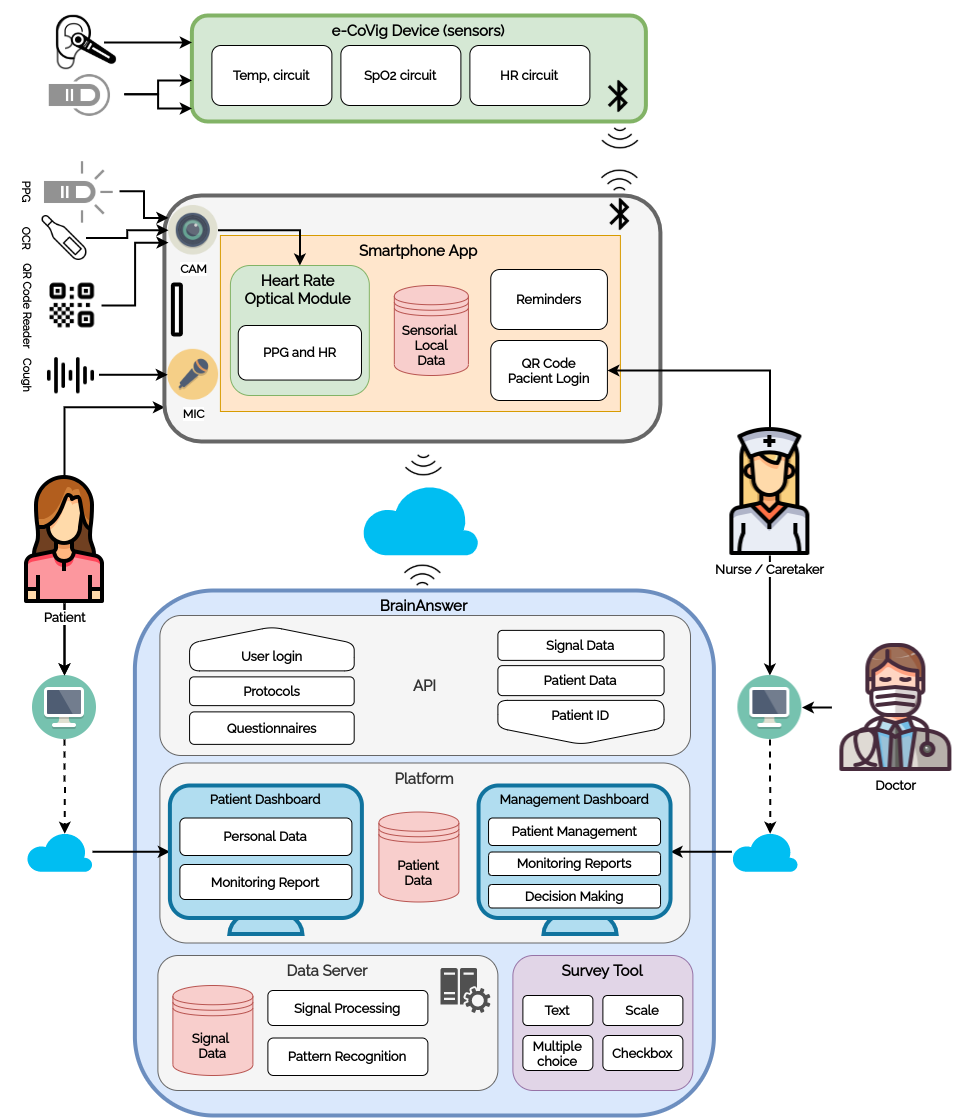
\includegraphics[width=0.60\linewidth]{images/ecovig.png}
    \caption[Diagram of e-Covig's system architecture.]{Overview of e-Covig's system architecture. Source: \cite{Raposo2021}.}
    \label{fig:ecovig-architecture}
\end{figure}


\subsection{Comparative Analysis}
% Quadro comparativo com maiores diferenças entre cada projeto e o WoW-WP4

\todo[inline]{To-do: Place table with a list of criteria to compare the different approaches.}

\subsection{Weaknesses of literature}

\subsubsection{Security and Privacy}

\todo[inline]{To-do: Complete section.}

\subsubsection{Interoperability}

Despite recent efforts, interoperability is still an issue of IoT systems. Due to the lack of clear and concise industry standards and regulations, many manufacturers push their own proprietary data formats and communication protocols, which hampers the integration of new resources since they are developed within closed ecosystems \cite{Rubi2019}. 
Moreover, the adoption of new systems can be often met with much objection from the clinical staff due to their mistrust of technology \cite{DursunErgezen2020}. 
In order to facilitate the integration of new systems, these should be easily 



%In context of healthcare solutions, PCHAlliance...
% PCHAlliance https://www.pchalliance.org/continua-design-guidelines 
%\begin{figure}[H]
%    \centering
%    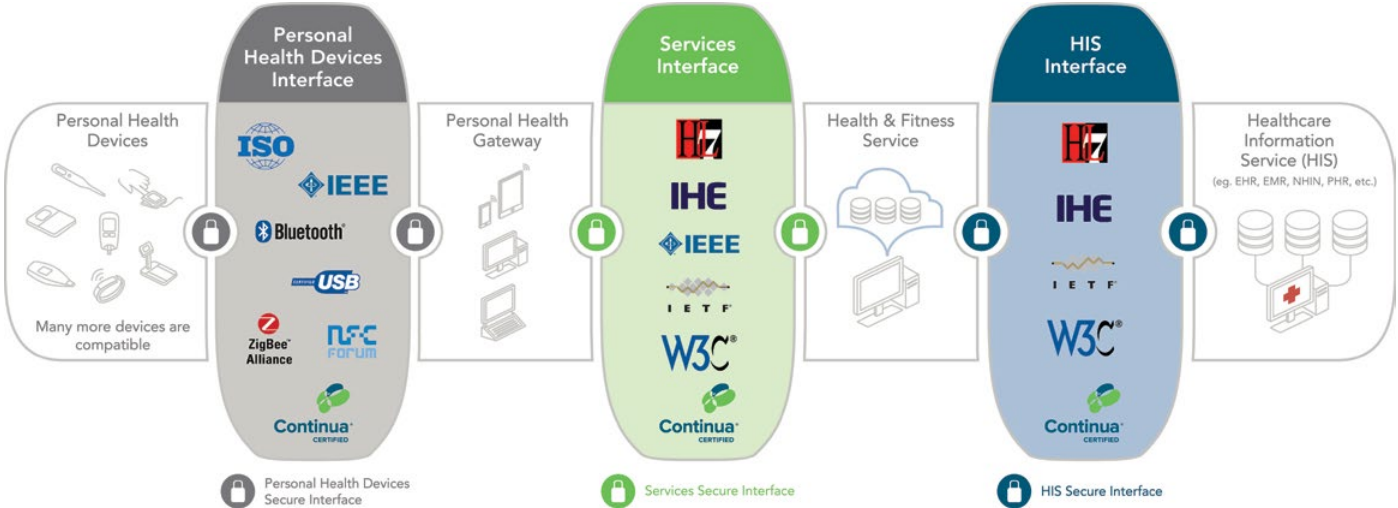
\includegraphics[width=.90\linewidth]{images/cdg-architecutre.png}
%    \caption{System architecture from the Personal Connected Health Alliance \cite{ContinuaHealthAlliance}.}
%    \label{fig:continua-architecture}
%\end{figure}

\section{Statement of Contributions}
%tendo em conta o estado da arte, as suas limitações e pontos fortes, propomos um sistema que
%1) vai para alem do estado da arte nisto e naquilo.
%2) inspira-se nos conceitos extistentes nisto e naquilo.

\todo[inline]{To-do: Complete section.}

After studying the different approaches taken by investigators, 
\begin{itemize}
    \item Hardware evaluation for edge nodes which integrate electronic wireless patches that gather patient's physiological signals;
    \item Integrating IoT system in an existing healthcare information system (Glintt GlobalCare software) through an FHIR API layer;
    \item Evaluation of the performance of the proposed system through a testbed and a real healthcare scenario;
\end{itemize}
